\documentclass[11pt, a4paper]{article}

\usepackage[utf8]{inputenc}
\usepackage[T1]{fontenc}
\usepackage[polish]{babel}
\usepackage{graphicx} 
\usepackage{geometry}
\usepackage{amsmath}
\usepackage{amsfonts}
\usepackage{amssymb}
\usepackage{float}
\usepackage{hyperref}
\usepackage{url}

\graphicspath{{images}}

\geometry{
  a4paper,
  total={170mm,257mm},
  left=20mm,
  top=20mm,
}

\title{Raport z Laboratorium 4 \\ \large Programowanie w Chmurze: REST API, JSON, Komunikacja z Serwerem}
\author{Mikołaj Kubś \\ 272662}
\date{\today}

\begin{document}
\maketitle
\begin{abstract}
Niniejszy raport podsumowuje realizację zadań w ramach Laboratorium 4, dotyczącego praktycznego wykorzystania REST API, formatu JSON oraz komunikacji klient-serwer. Opracowano dwie aplikacje: klienta API pogodowego oraz system klient-serwer do zarządzania listą albumów muzycznych.
\end{abstract}

\section{Wprowadzenie}
Laboratorium miało na celu zapoznanie studentów z fundamentalnymi koncepcjami związanymi z architekturą REST, formatem wymiany danych JSON oraz implementacją komunikacji sieciowej. Zadania obejmowały zarówno konsumpcję zewnętrznego API, jak i tworzenie własnego serwera REST API.

\section{Zadanie 1: Aplikacja Pogodowa z OpenWeatherMap}
\subsection{Cel zadania}
Celem zadania było stworzenie aplikacji klienckiej w technologii React, która pobiera i wyświetla dane pogodowe z serwisu OpenWeatherMap dla wskazanej przez użytkownika lokalizacji lub na podstawie geolokalizacji.

\subsection{Realizacja}
Aplikacja została zaimplementowana zgodnie z wytycznymi. Kluczowe etapy realizacji obejmowały:
\begin{itemize}
    \item Rejestrację w serwisie OpenWeatherMap i uzyskanie klucza API.
    \item Stworzenie komponentu React z interfejsem użytkownika umożliwiającym wprowadzenie nazwy miasta.
    \item Implementację funkcji asynchronicznej do wysyłania żądania GET do API OpenWeatherMap.
    \item Przetwarzanie odpowiedzi JSON i wyświetlanie danych pogodowych.
    \item Dodanie obsługi geolokalizacji oraz dynamiczne dostosowanie wyglądu aplikacji (np. tła, ikon) do aktualnych warunków pogodowych.
    \item Użycie pliku .env do przechowywania sekretów.
\end{itemize}

\begin{figure}[H]
    \centering
    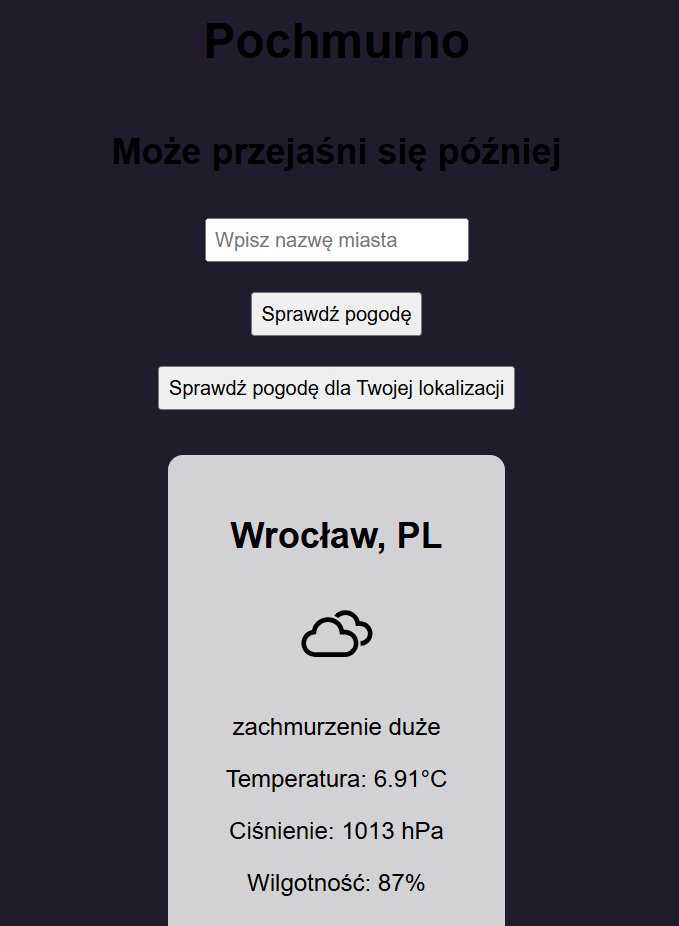
\includegraphics[width=0.8\textwidth]{weather-location.png}
    \caption{Interfejs użytkownika aplikacji pogodowej - pogoda dla lokalizacji.}
    \label{fig:pogoda_ui}
\end{figure}

\begin{figure}[H]
    \centering
    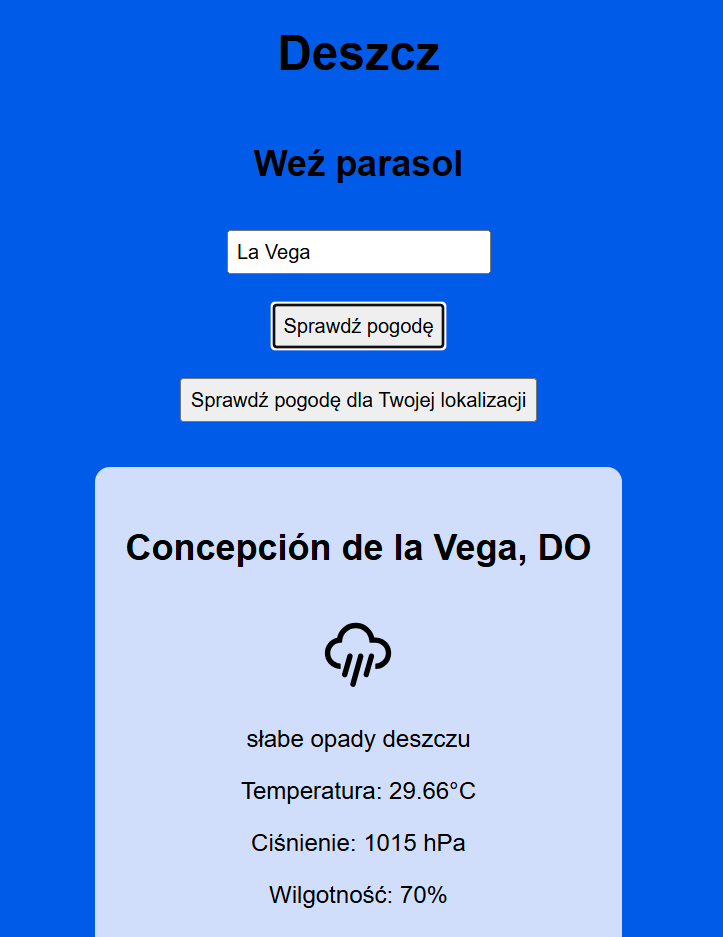
\includegraphics[width=0.8\textwidth]{weather-city.png}
    \caption{Wyświetlanie danych pogodowych dla przykładowego miasta.}
    \label{fig:pogoda_wynik}
\end{figure}

\section{Zadanie 2: Własny Serwer REST API i Klient}
\subsection{Cel zadania}
Zadanie polegało na zbudowaniu prostego serwera REST API w Node.js z użyciem frameworka Express, serwującego dane o albumach muzycznych, oraz aplikacji klienckiej w React do interakcji z tym API (operacje CRUD).

\subsection{Realizacja - Serwer (Node.js/Express)}
Serwer został zaimplementowany w Node.js przy użyciu Express. Główne funkcjonalności serwera:
\begin{itemize}
    \item Definicja danych (lista albumów) przechowywanych w pamięci serwera.
    \item Endpointy REST API:
    \begin{itemize}
        \item \texttt{GET /albums} - pobranie wszystkich albumów.
        \item \texttt{GET /genres} - pobranie wszystkich gatunków.
        \item \texttt{GET /albums/:band} - pobranie albumów danego zespołu.
        \item \texttt{POST /albums} - dodanie nowego albumu.
        \item \texttt{PUT /albums/:id} - aktualizacja danych albumu.
        \item \texttt{DELETE /albums/:id} - usunięcie albumu.
    \end{itemize}
    \item Proste testy podstawowej funkcjonalności backendu.    
    \item Dodanie cover i genre - zdjęć okładki przechowywanych na serwerze i zapisywanych po dodaniu z formularza i możliwość wyboru gatunku jako dropdown. 
\end{itemize}

\begin{figure}[H]
    \centering
    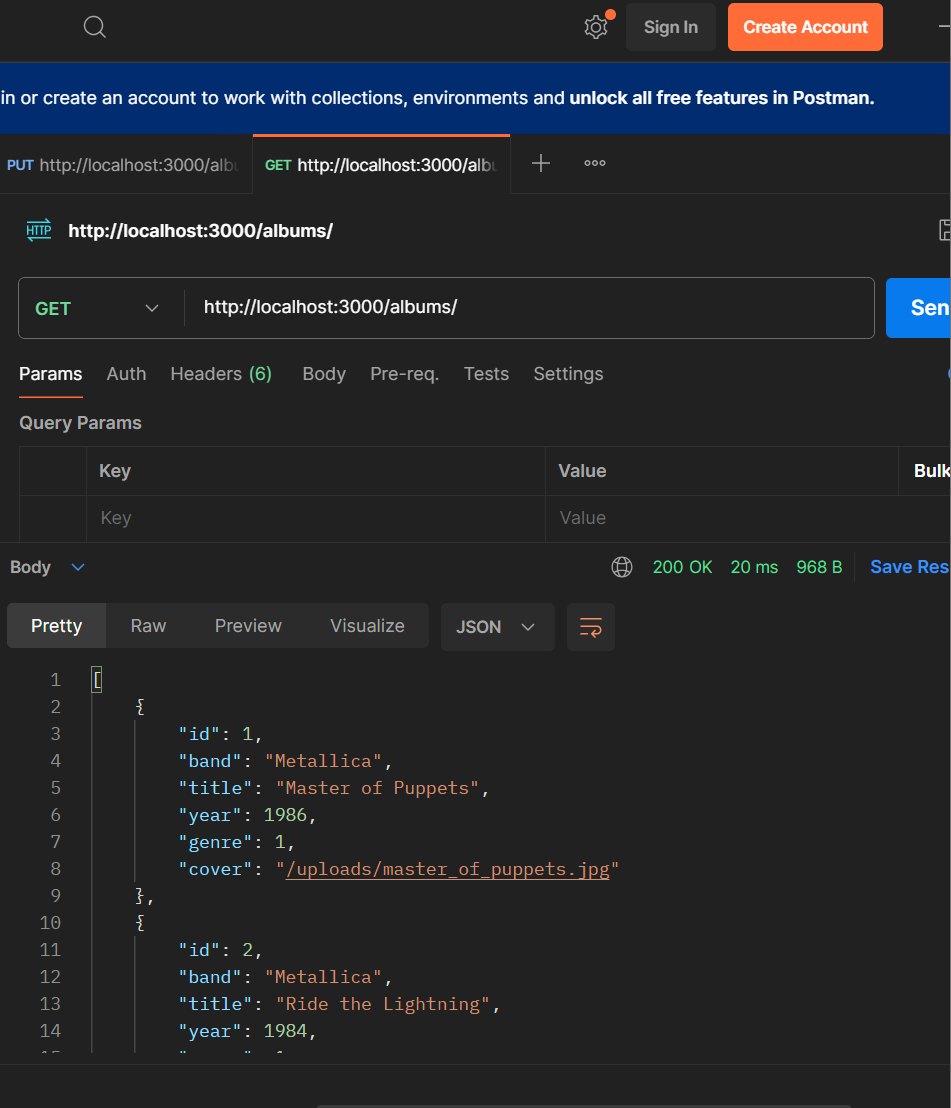
\includegraphics[width=0.7\textwidth]{postman.png}
    \caption{Testowanie endpointu serwera API w Postman.}
    \label{fig:serwer_test}
\end{figure}

\subsection{Realizacja - Klient (React)}
Aplikacja kliencka w React została stworzona do interakcji z serwerem API.
\begin{itemize}
    \item Implementacja komponentu do wyświetlania listy albumów.
    \item Funkcje do pobierania, dodawania, edycji i usuwania albumów poprzez wysyłanie żądań HTTP do serwera.
    \item Interfejs użytkownika umożliwiający zarządzanie kolekcją albumów.
    \item Wykorzystanie \texttt{localStorage} do buforowania danych.
    \item Dodanie cover i genre - zdjęć okładki przechowywanych na serwerze i zapisywanych po dodaniu z formularza i możliwość wyboru gatunku jako dropdown. 
    \item Jasny i ciemny tryb z custom Switch.
\end{itemize}

\begin{figure}[H]
    \centering
    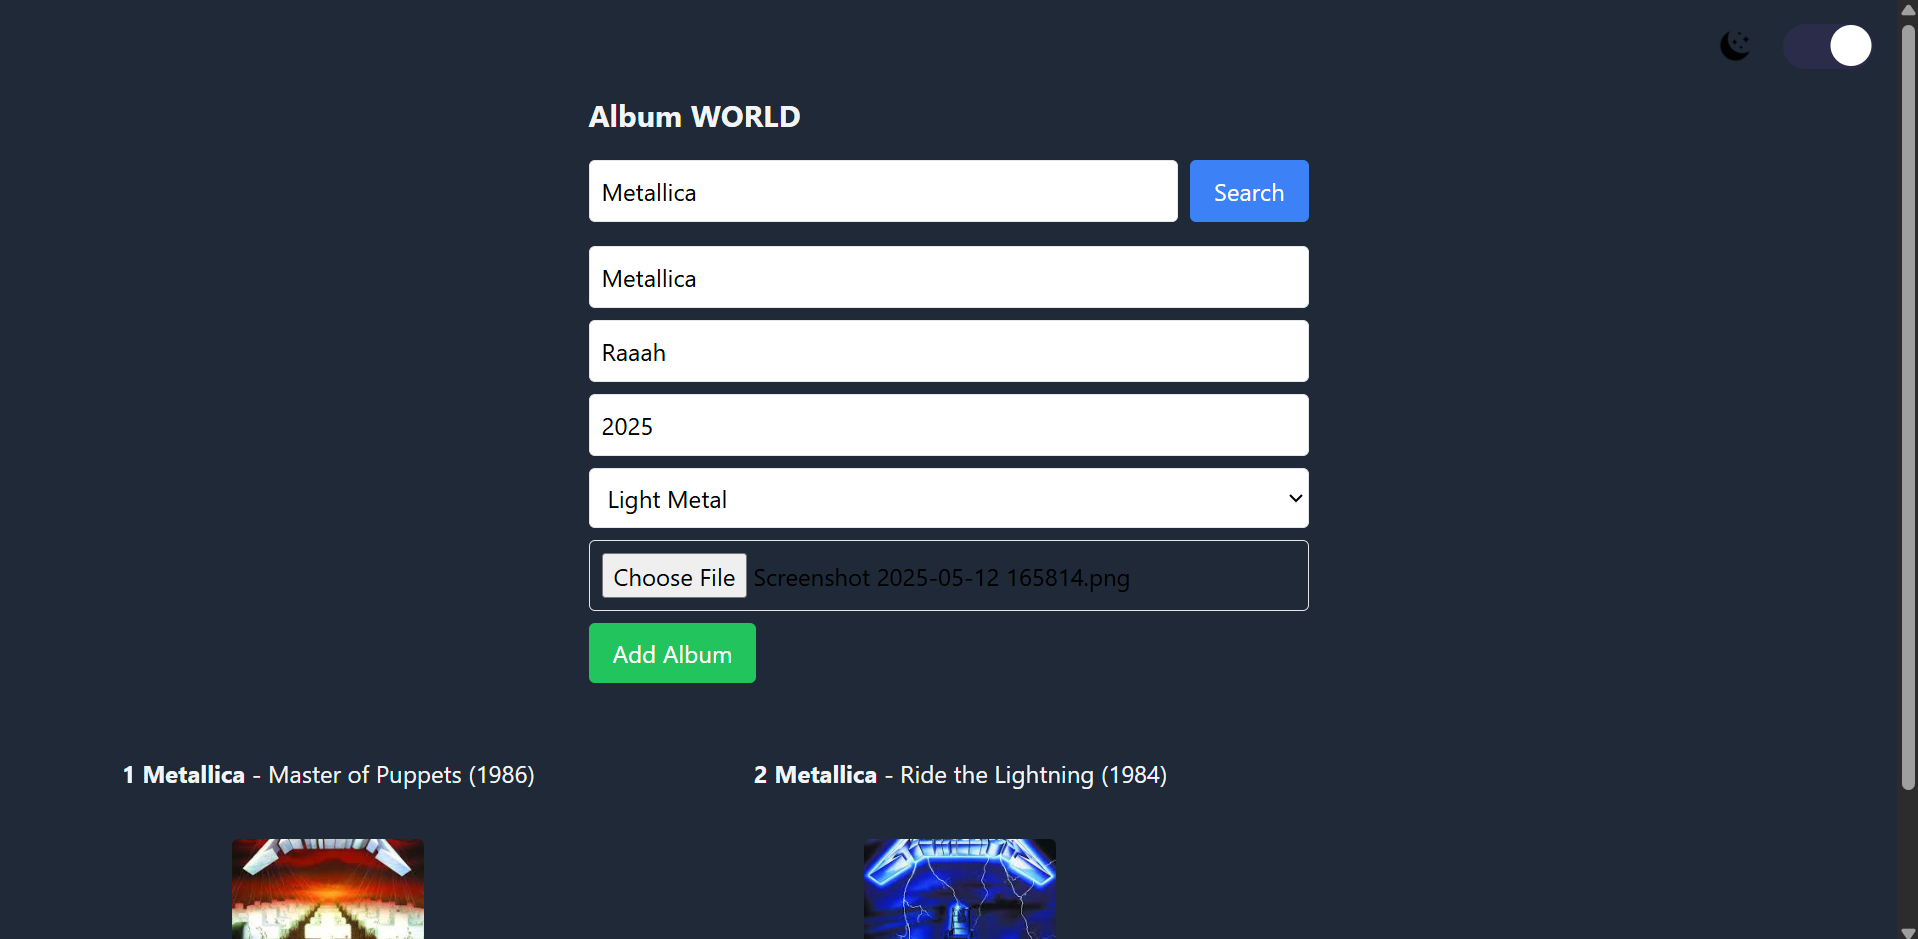
\includegraphics[width=0.8\textwidth]{album-main.png}
    \caption{Formularz tworzenia albumu.}
\end{figure}

\begin{figure}[H]
    \centering
    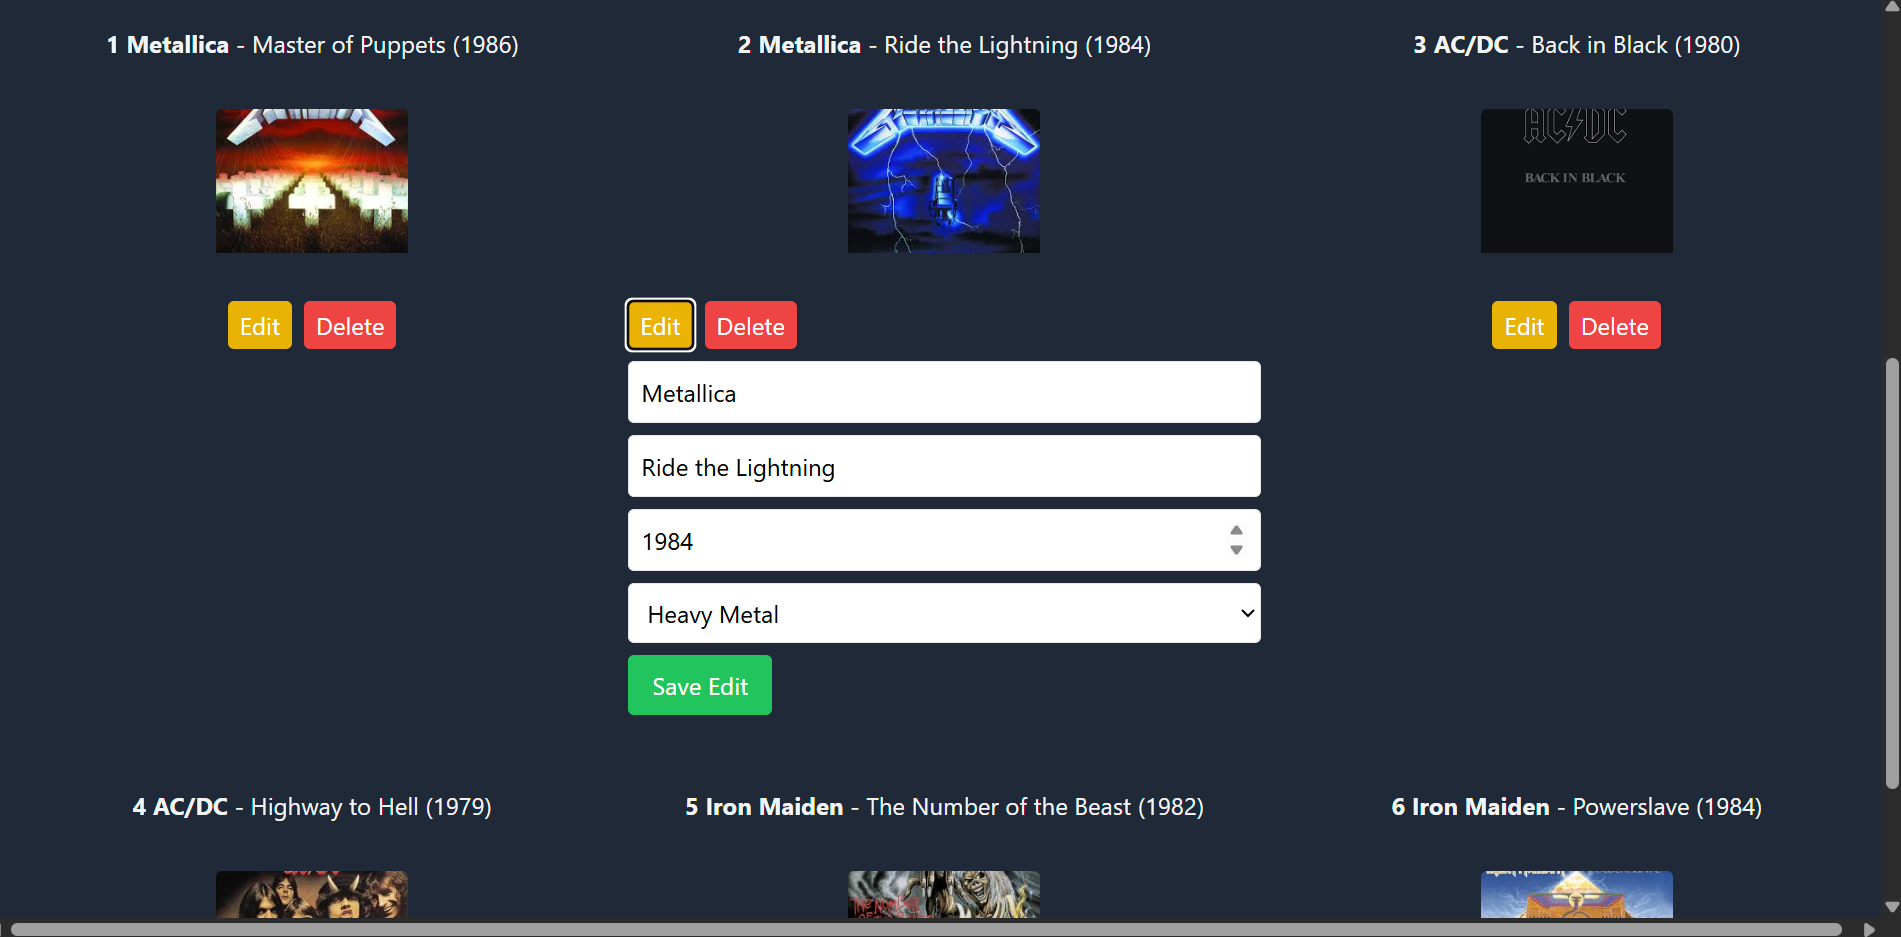
\includegraphics[width=0.7\textwidth]{album-edit.png}
    \caption{Formularz edycji albumu.}
\end{figure}

\begin{figure}[H]
    \centering
    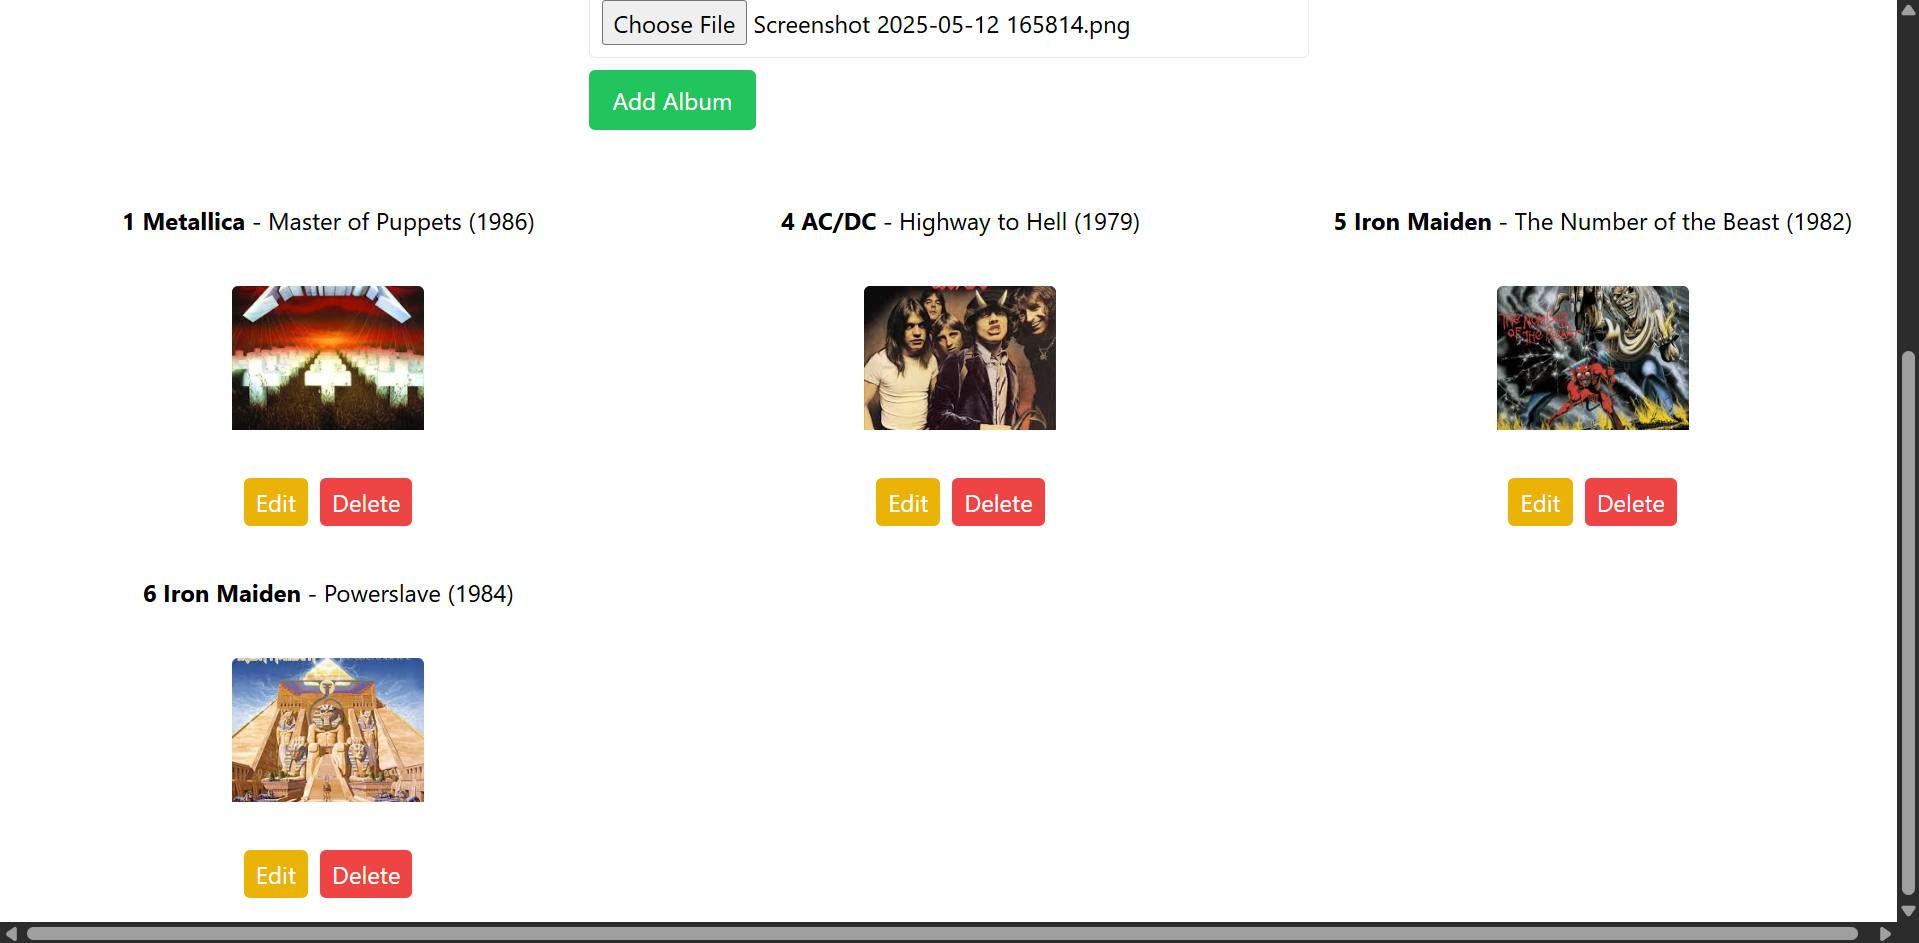
\includegraphics[width=0.7\textwidth]{album-light.png}
    \caption{Widok aplikacji w trybie jasnym.}
\end{figure}

\section{Podsumowanie}
Laboratorium pozwoliło na praktyczne zastosowanie wiedzy dotyczącej REST API i formatu JSON. Zrealizowane zadania umożliwiły przećwiczenie procesu tworzenia aplikacji komunikujących się z serwerami za pomocą protokołu HTTP, zarówno w roli konsumenta istniejącego API, jak i twórcy własnego serwisu REST. Zdobyte umiejętności są kluczowe w nowoczesnym tworzeniu aplikacji webowych i mobilnych.

\section{Link do repozytorium}
Kod źródłowy aplikacji oraz instrukcje uruchomienia dostępne są w repozytorium GitHub: \\
\url{https://github.com/lmProgramming/uni-cloud-development}

\end{document}